\section{Wprowadzenie}

\begin{frame}
     \frametitle{Domain Specific Languages (DSL)}
     
     DSL to języki przystosowane do używania w konkretnym celu.
     \begin{itemize}
          \item
          łatwość użycia
          \item
          specyficzne konstrukcje
          \item 
          ograniczone możliwości
          \item
          kompilacja do języka niższego poziomu (np. SQL)
     \end{itemize}


\end{frame}



\begin{frame}
\frametitle{Sumerologia}
\begin{columns}
 \column{0.5\textwidth}
Sumerologia to nauka badająca kulturę i historię starożytnych Sumerów, czerpiąca wiedzę m.in. z zachowanych tabliczek.
\begin{itemize}
\item zdigitalizowane i ręcznie skorygowane treści tabliczek są udostępnione przez system CDLI (obecnie prawie 225 000 tabliczek)
\item możliwość niewłaściwej interpretacji klinów
\item potrzebne intuicyjne narzędzie do wyszukiwania w bazie tabliczek na podstawie odczytów
\end{itemize} 
 \column{0.5\textwidth}
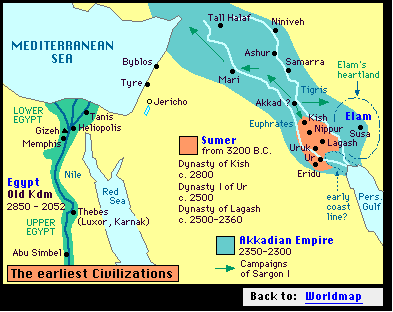
\includegraphics[width=55mm]{../1/sum_map.png}
\end{columns}
\end{frame}


\begin{frame}
\frametitle{Dane z CDLI}
\begin{columns}
 \column{0.5\textwidth}
 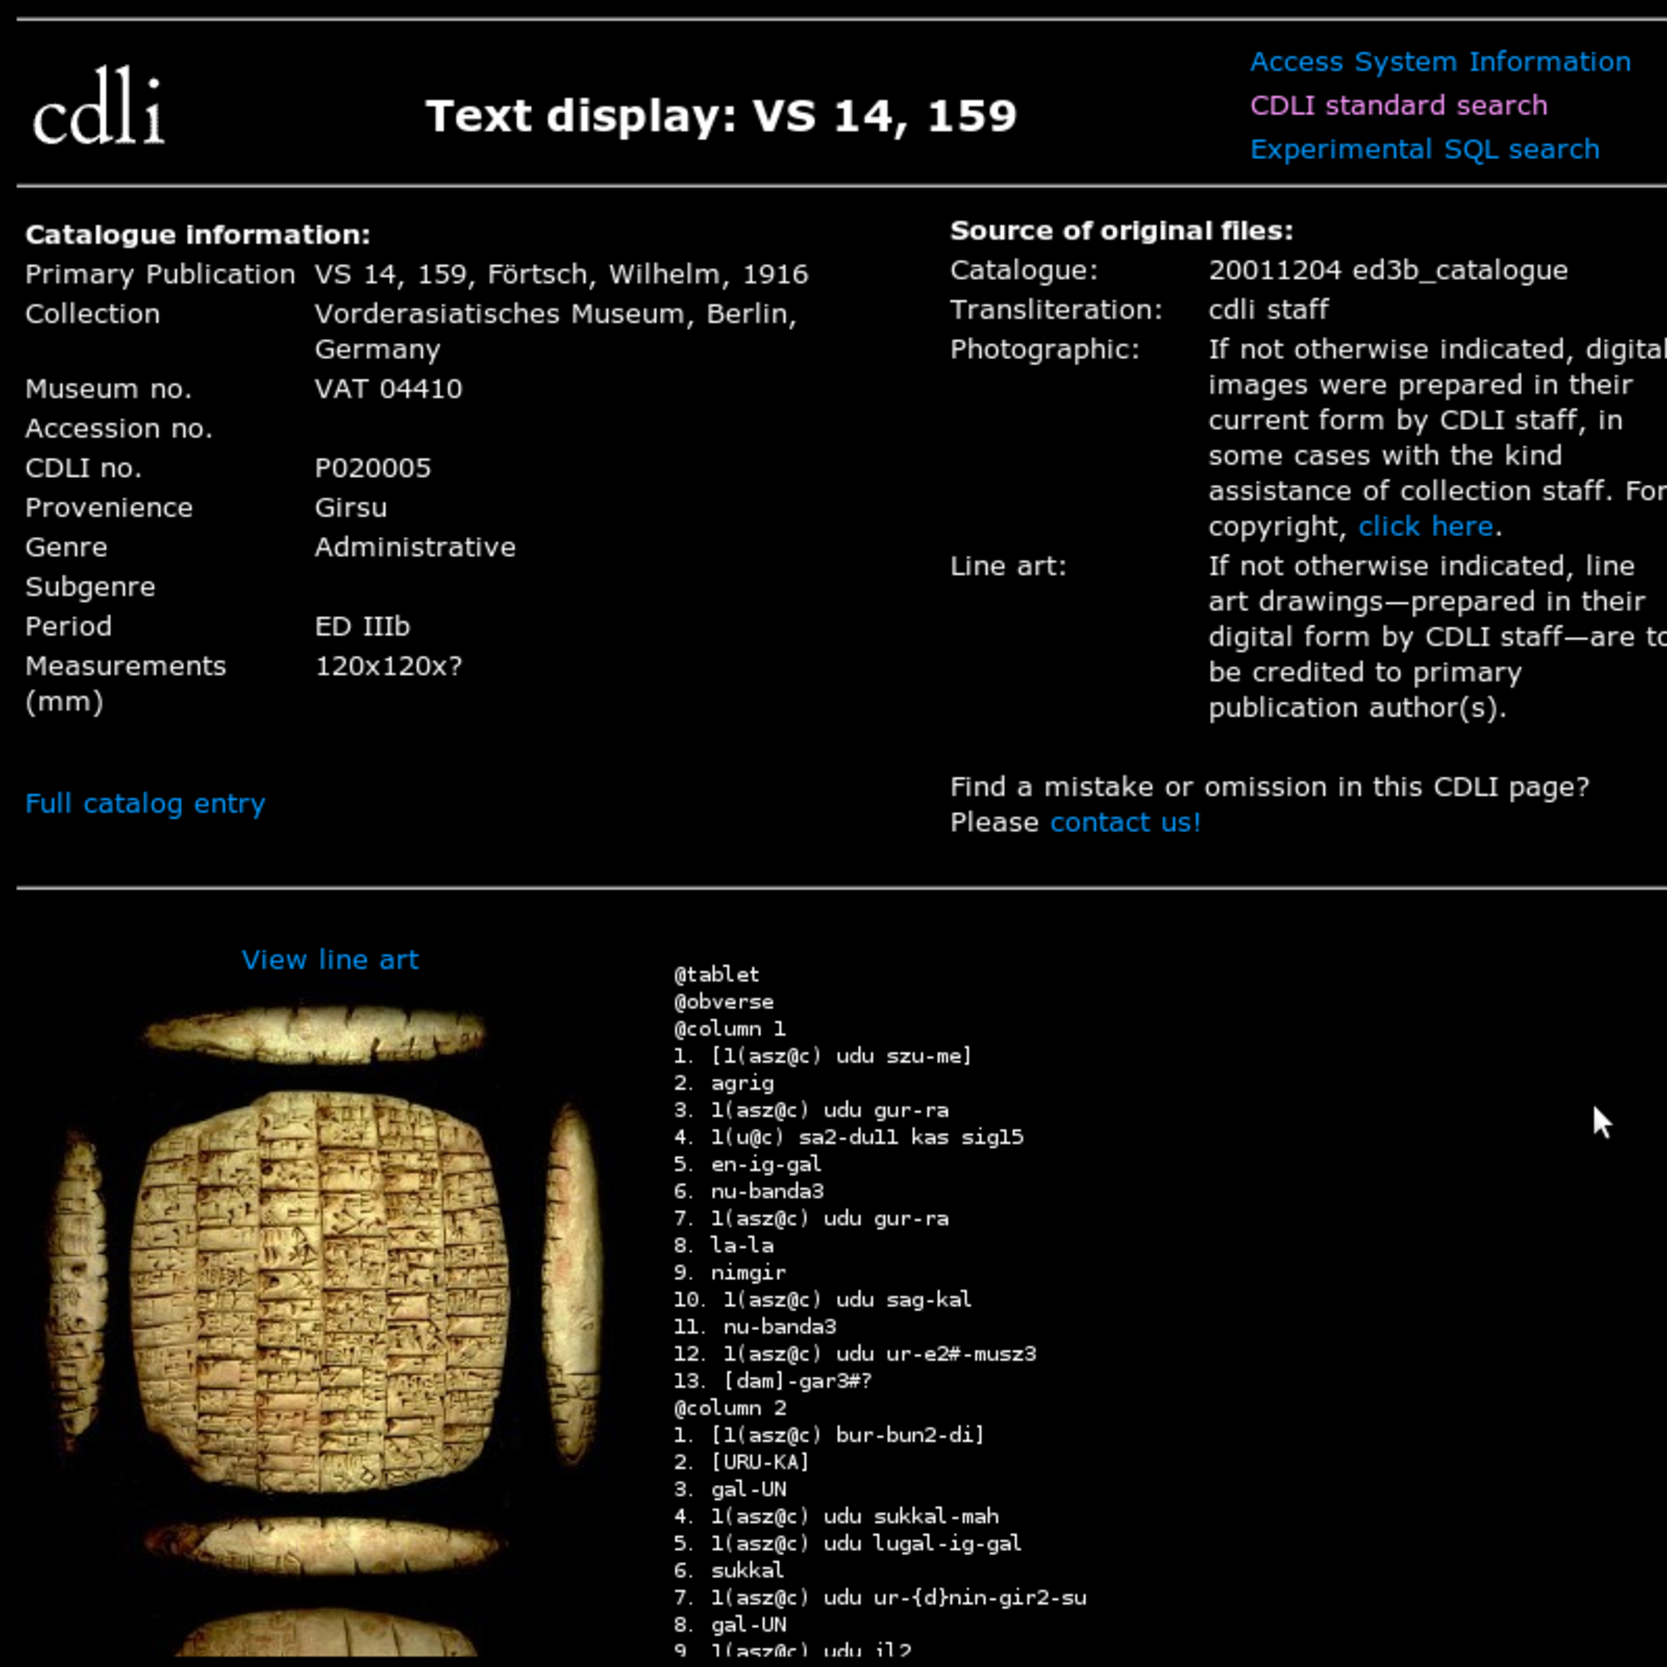
\includegraphics[width=55mm]{../diagramy/cdli.pdf}      
 \column{0.5\textwidth}
\begin{block}{Treść tabliczki}
@tablet \\
@obverse \\
@column 1 \\
1. [1(asz@c) udu szu-me] \\
2. agrig \\
3. 1(asz@c) udu gur-ra \\
4. 1(u@c) sa2-du11 kas sig15 \\
5. en-ig-gal \\
6. nu-banda3 \\
7. 1(asz@c) udu gur-ra \\
8. la-la \\
9. nimgir \\
10. 1(asz@c) udu sag-kal \\
11. nu-banda3 \\
% 12. 1(asz@c) udu ur-e2#-musz3 \\
% 13. [dam]-gar3#? \\
% @column 2 \\
% 1. [1(asz@c) bur-bun2-di] \\
% 2. [URU-KA] \\
% 3. gal-UN \\
% 4. 1(asz@c) udu sukkal-mah \\
% 5. 1(asz@c) udu lugal-ig-gal \\
% 6. sukkal \\
% 7. 1(asz@c) udu ur-{d}nin-gir2-su \\
% 8. gal-UN \\
% 9. 1(asz@c) udu il2 \\
% 10. gal-UN \\
% 11. 1(asz@c) udu \\
% 12. lam-sag-du3 \\
% 13. mu6-sub3 \\
% 14. 1(asz@c) masz lugud2-da \\
% 15. dun-dun \\
% @column 3 \\
% 1. gal-UN \\
% 2. 1(asz@c) udu ur-ki \\
% 3. gal-UN \\
% 4. 1(u@c) mudx(LAK449) kas ge6 \\
% 5. 1(u@c) sa2-du11 kas sig15 \\
% 6. 5(gesz2@c) ninda gir2 \\
% 7. 1(gesz'u@c) ninda siki2 sze \\
% 8. 1(asz@c) udu 1(asz@c) masz \\
% 9. dub-sar-mah \\
% 10. 1(asz@c) masz geszgal-si \\
% 11. gal-UN \\
% 12. 1(asz@c) udu \\
% 13. amar-ezem \\
% 14. nu-banda3 \\
% 15. 1(asz@c) udu \\
% 16. szul-szesz \\
\end{block}

\end{columns}
\end{frame}

\begin{frame}
     \frametitle{Tablets Query Language}
 \begin{columns}
 \column{0.5\textwidth}
   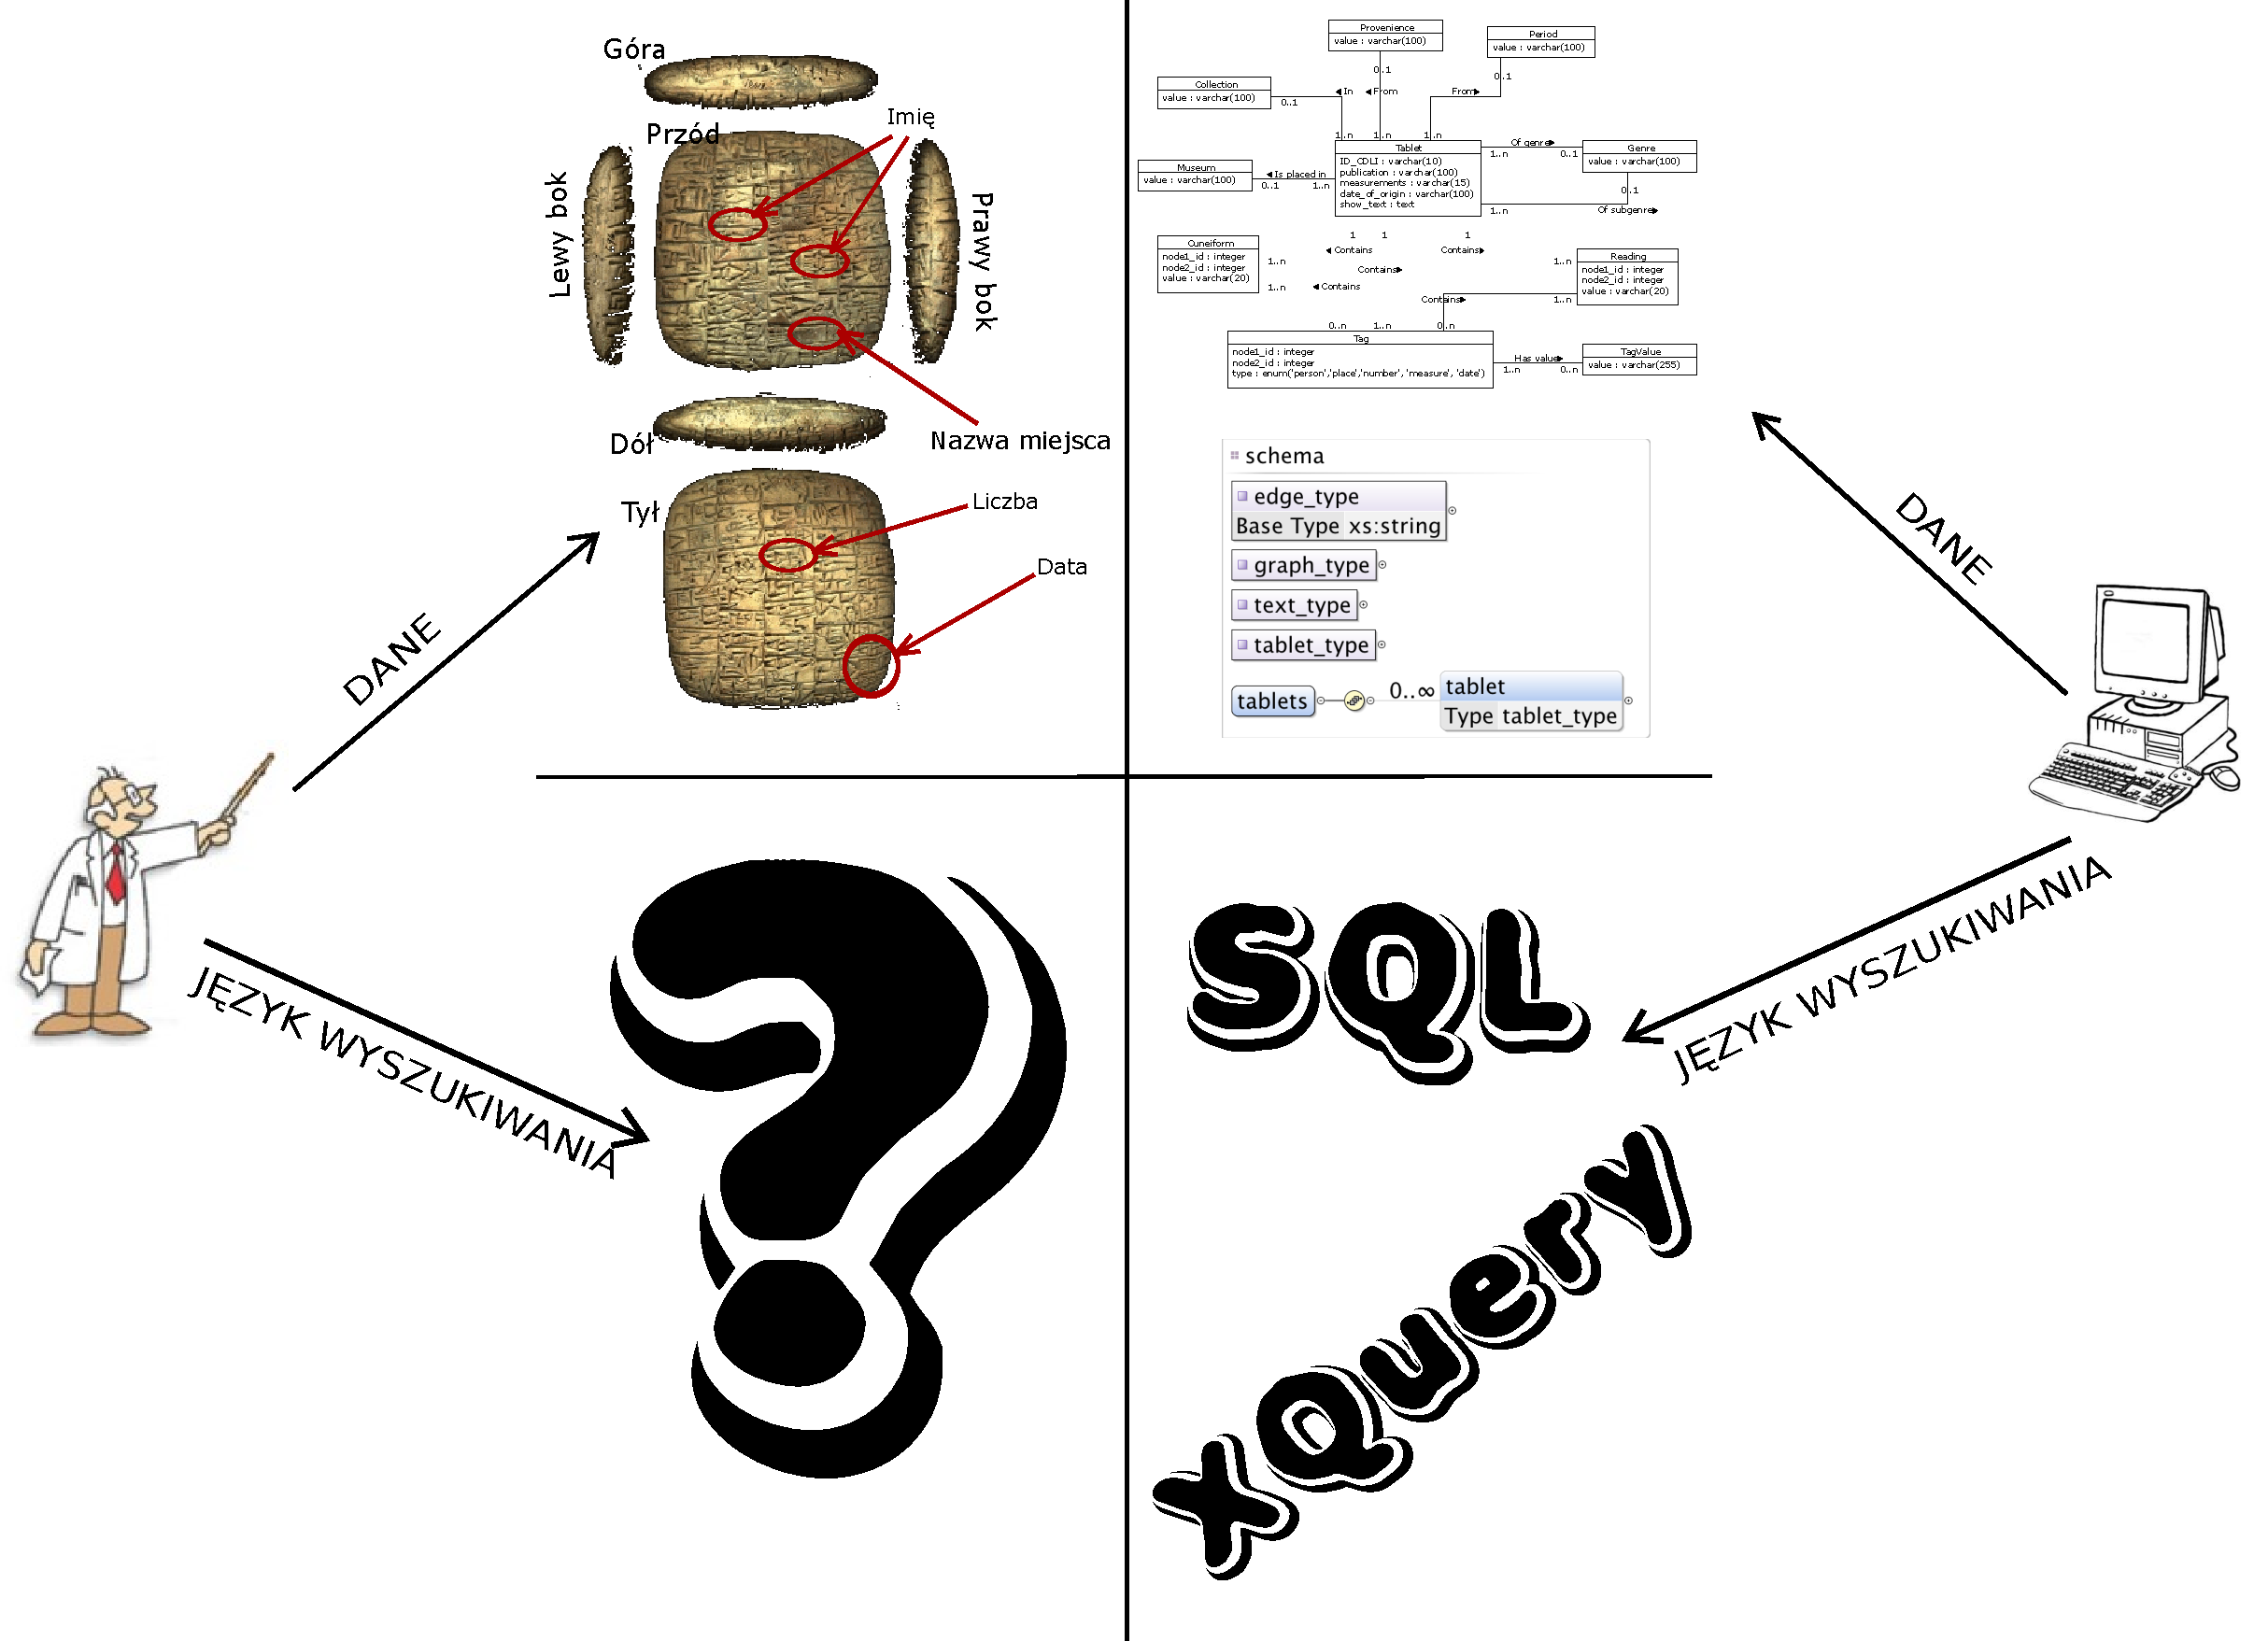
\includegraphics[width=55mm]{../diagramy/poco.pdf}      
 \column{0.5\textwidth}
  \begin{itemize}
    \item Język pozwalający sumerologom łatwo tworzyć zapytania w bazie tabliczek.\\
    \item  Prosta składnia zapytań.\\
    \item    Zapytania zawierają informacje tylko o treści tabliczek i ich metadanych.\\
    \item   Możliwość stworzenia implementacji na dowolną bazę przechowującą tabliczki.\\ %ułatwiamy to dzięki podziałowi kodu na moduły
  \end{itemize}
 \end{columns}
\end{frame}

\begin{frame}
 \frametitle{Przykładowe zapytanie TQL}
\begin{block}{Przykład}
\textbf{define}\\
~~provenience: Garshana\\
~~text: "udu ban"/mash2\\
\textbf{as} "zwierzaki w Garshana"\\
~\\
\textbf{search}\\
~~period: UrIII\\
~~text: szid + sipa $--$ adad-tilati\\
\textbf{in} "zwierzaki w Garshana"\\
~\\
\textbf{search}\\
~~period: UrIV\\
~~genre: Adm*\\
\textbf{in} "zwierzaki w Garshana"\\
\end{block}
\end{frame}
